\addtolength{\oddsidemargin}{-.900in}\addtolength{\evensidemargin}{-.900in}
\addtolength{\textwidth}{1.75in}
\addtolength{\topmargin}{-.875in}
\addtolength{\textheight}{1.75in}
\documentclass[12pt]{homework}

\newcommand{\hwname}{Ornella Elena Grassi}
\newcommand{\hwemail}{s290310@studenti.polito.it}
\newcommand{\hwtype}{Homework}
\newcommand{\hwnum}{1}
\newcommand{\hwclass}{}
\newcommand{\hwlecture}{}
\newcommand{\hwsection}{}
\DeclareMathOperator*{\slim}{s-lim}

% This is just used to generate filler content. You don't need it in an actual
% homework!
\usepackage{lipsum}
\usepackage{amssymb}
\usepackage[utf8]{inputenc}
\usepackage[T1]{fontenc}
\usepackage{lmodern}
\usepackage{amsfonts}
\usepackage{hyperref}
\usepackage{bbm}
\usepackage{amsmath}
\usepackage{mcode}
\usepackage{epstopdf}
\usepackage{subcaption}
\usepackage[italian]{babel}
\usepackage{ stmaryrd }
\usepackage{bbm}
%usepackage{geometry}
\begin{document}
\maketitle
\begin{center}
Realizzato in collaborazione con Giulio Nenna (s245717), Andrea Sanna (s222975) e Alfredo Baione (s279328)
\end{center}
\section{}
% --------------ESERCIZIO1------------------------------
\begin{enumerate}


  
    \item
    Se una catena di Markov a stati finiti è irriducibile, allora tutti i suoi stati sono ricorrenti, ovvero
    \begin{equation*}
    \mathbb{E}_{i}[T_{i}]=\mathbb{E}[T_{i}\mid X_{0}=i]<\infty,
    \end{equation*}
    cioè il tempo medio di primo ritorno in $i$ è minore di $\infty$.\\
    Inoltre sappiamo che, per questa catena, esiste un'unica distribuzione stazionaria e che, in generale, una distribuzione limite è una distribuzione stazionaria.\\
    Dunque, in questo particolare caso, basterà scegliere due catene di Markov a tempo discreto le cui matrici di transizione siano doppiamente stocastiche e aperiodiche (condizione che garantisce l'esistenza di una distribuzione limite nel nostro caso), ad esempio
    \begin{align*}
    p_{1}=\begin{bmatrix}
        \frac{1}{2} & \frac{1}{2}\\
        \frac{1}{2} & \frac{1}{2} \\ 
      \end{bmatrix}, &&  
      p_{2}=\begin{bmatrix}
         0.4 & 0.6\\
        0.6 & 0.4 \\ 
      \end{bmatrix}
    \end{align*}
    
    e osservare che, per questi due processi, indipendentemente dallo stato iniziale, la distribuzione uniforme è sempre una distribuzione stazionaria. \\
    Si avrà
    \begin{equation*}
    \pi_{S}\left(1\right)=\pi_{S}\left(2\right)= \left(\frac{1}{2},\frac{1}{2}\right)'
    \end{equation*}
     e questa sarà anche la loro distribuzione limite.
     \newpage
     
     \item
     Due DTMC a stati finiti, diverse, che ammettono la stessa distribuzione stazionaria e la stessa distribuzione limite, potrebbero essere due catene siffatte:
     
     \begin{figure}[htb]\centering
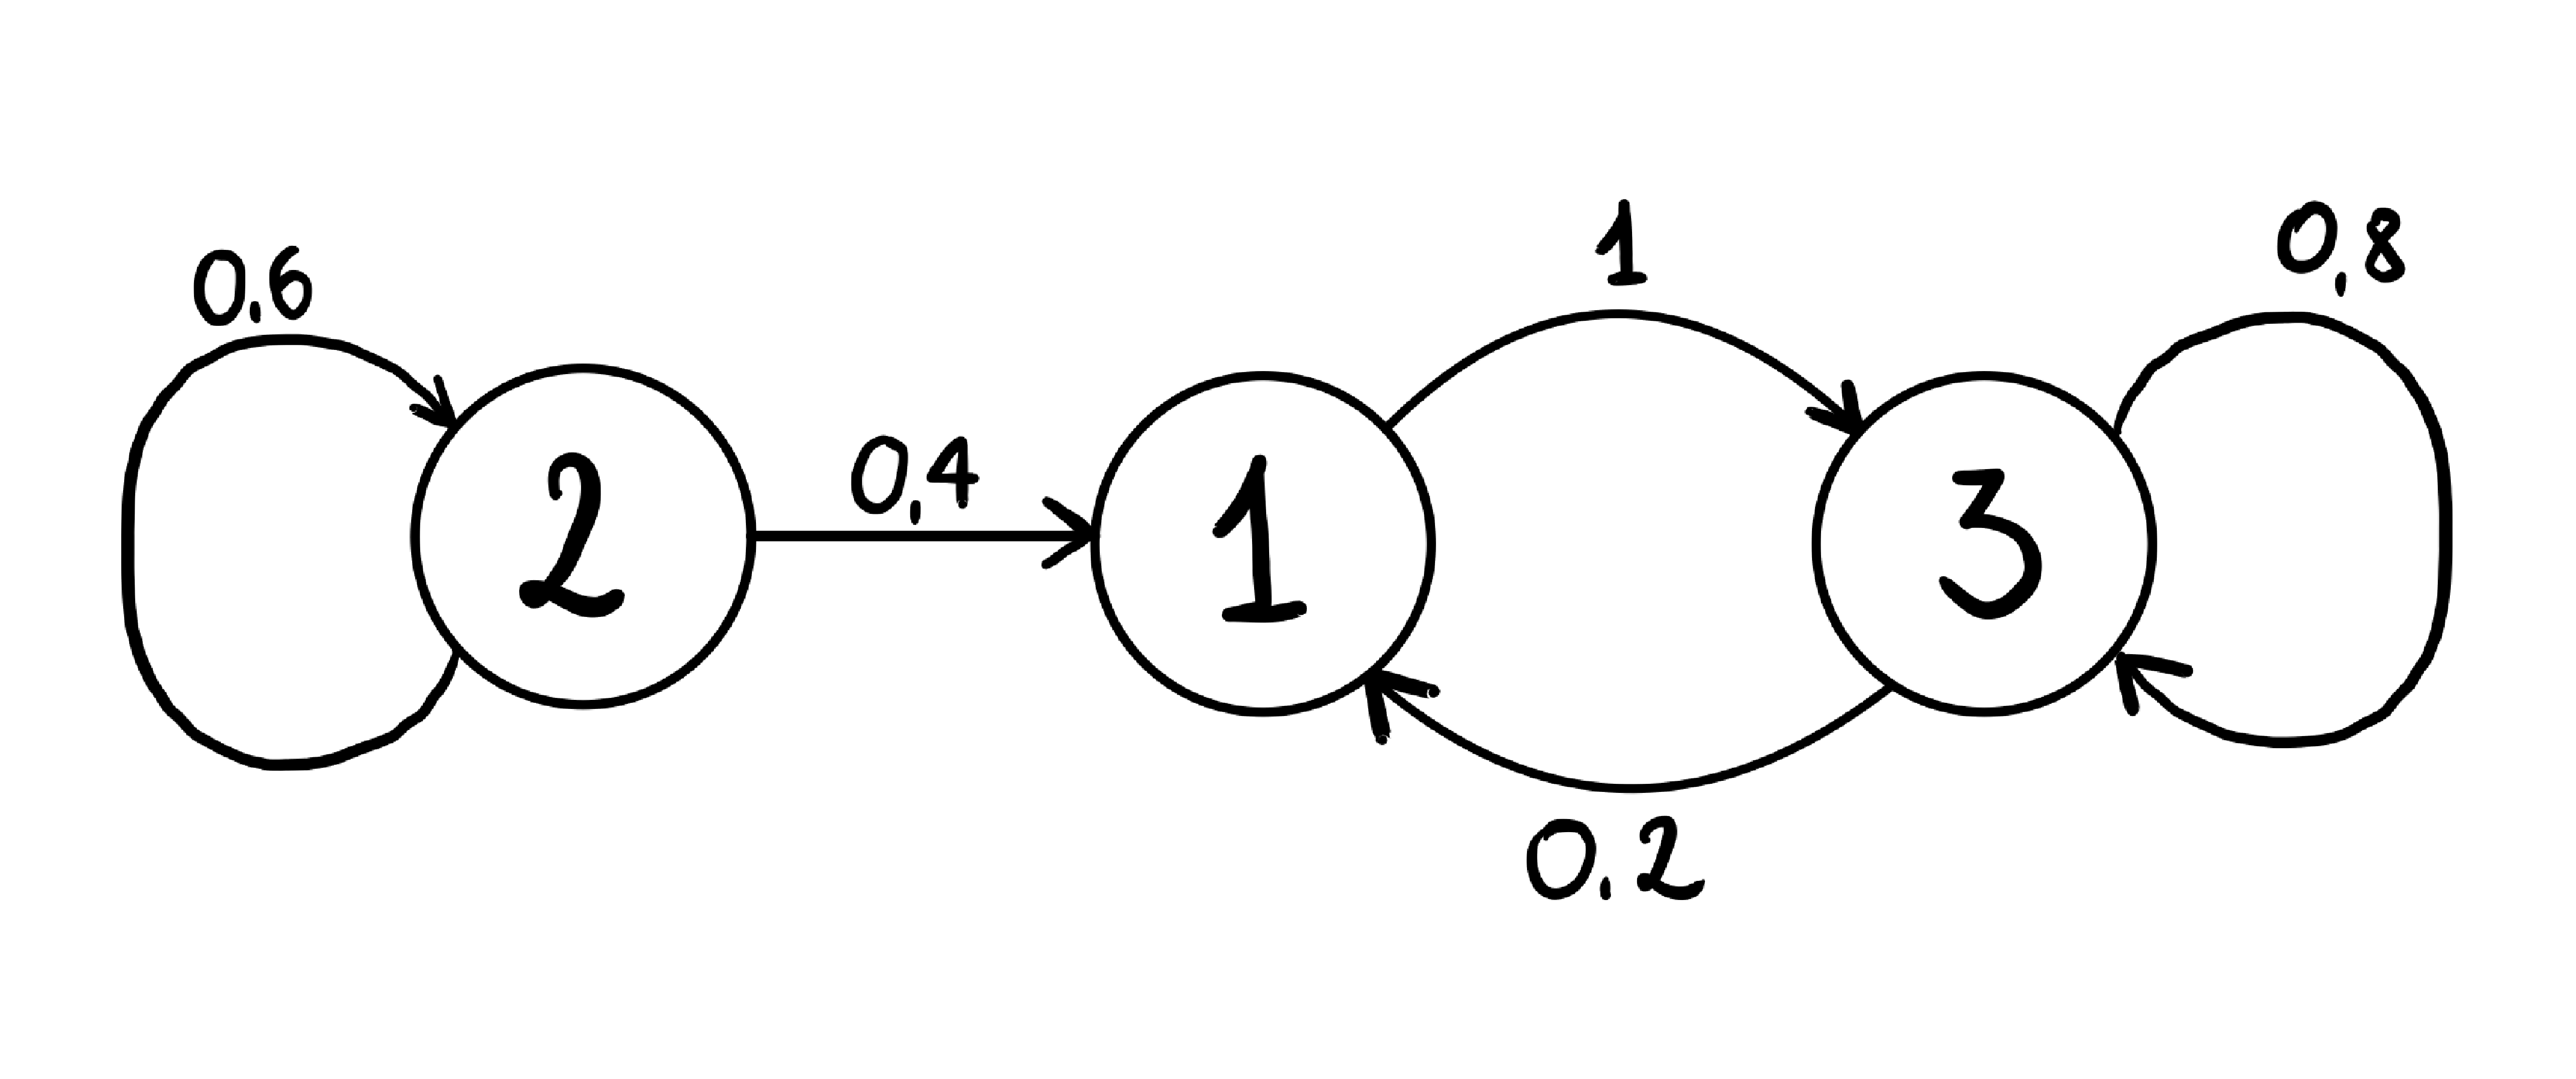
\includegraphics[scale=0.08]{Catena2.1.eps}
\captionof{figure}{Catena 1.}
  \end{figure}
      
     \begin{figure}[htb]\centering
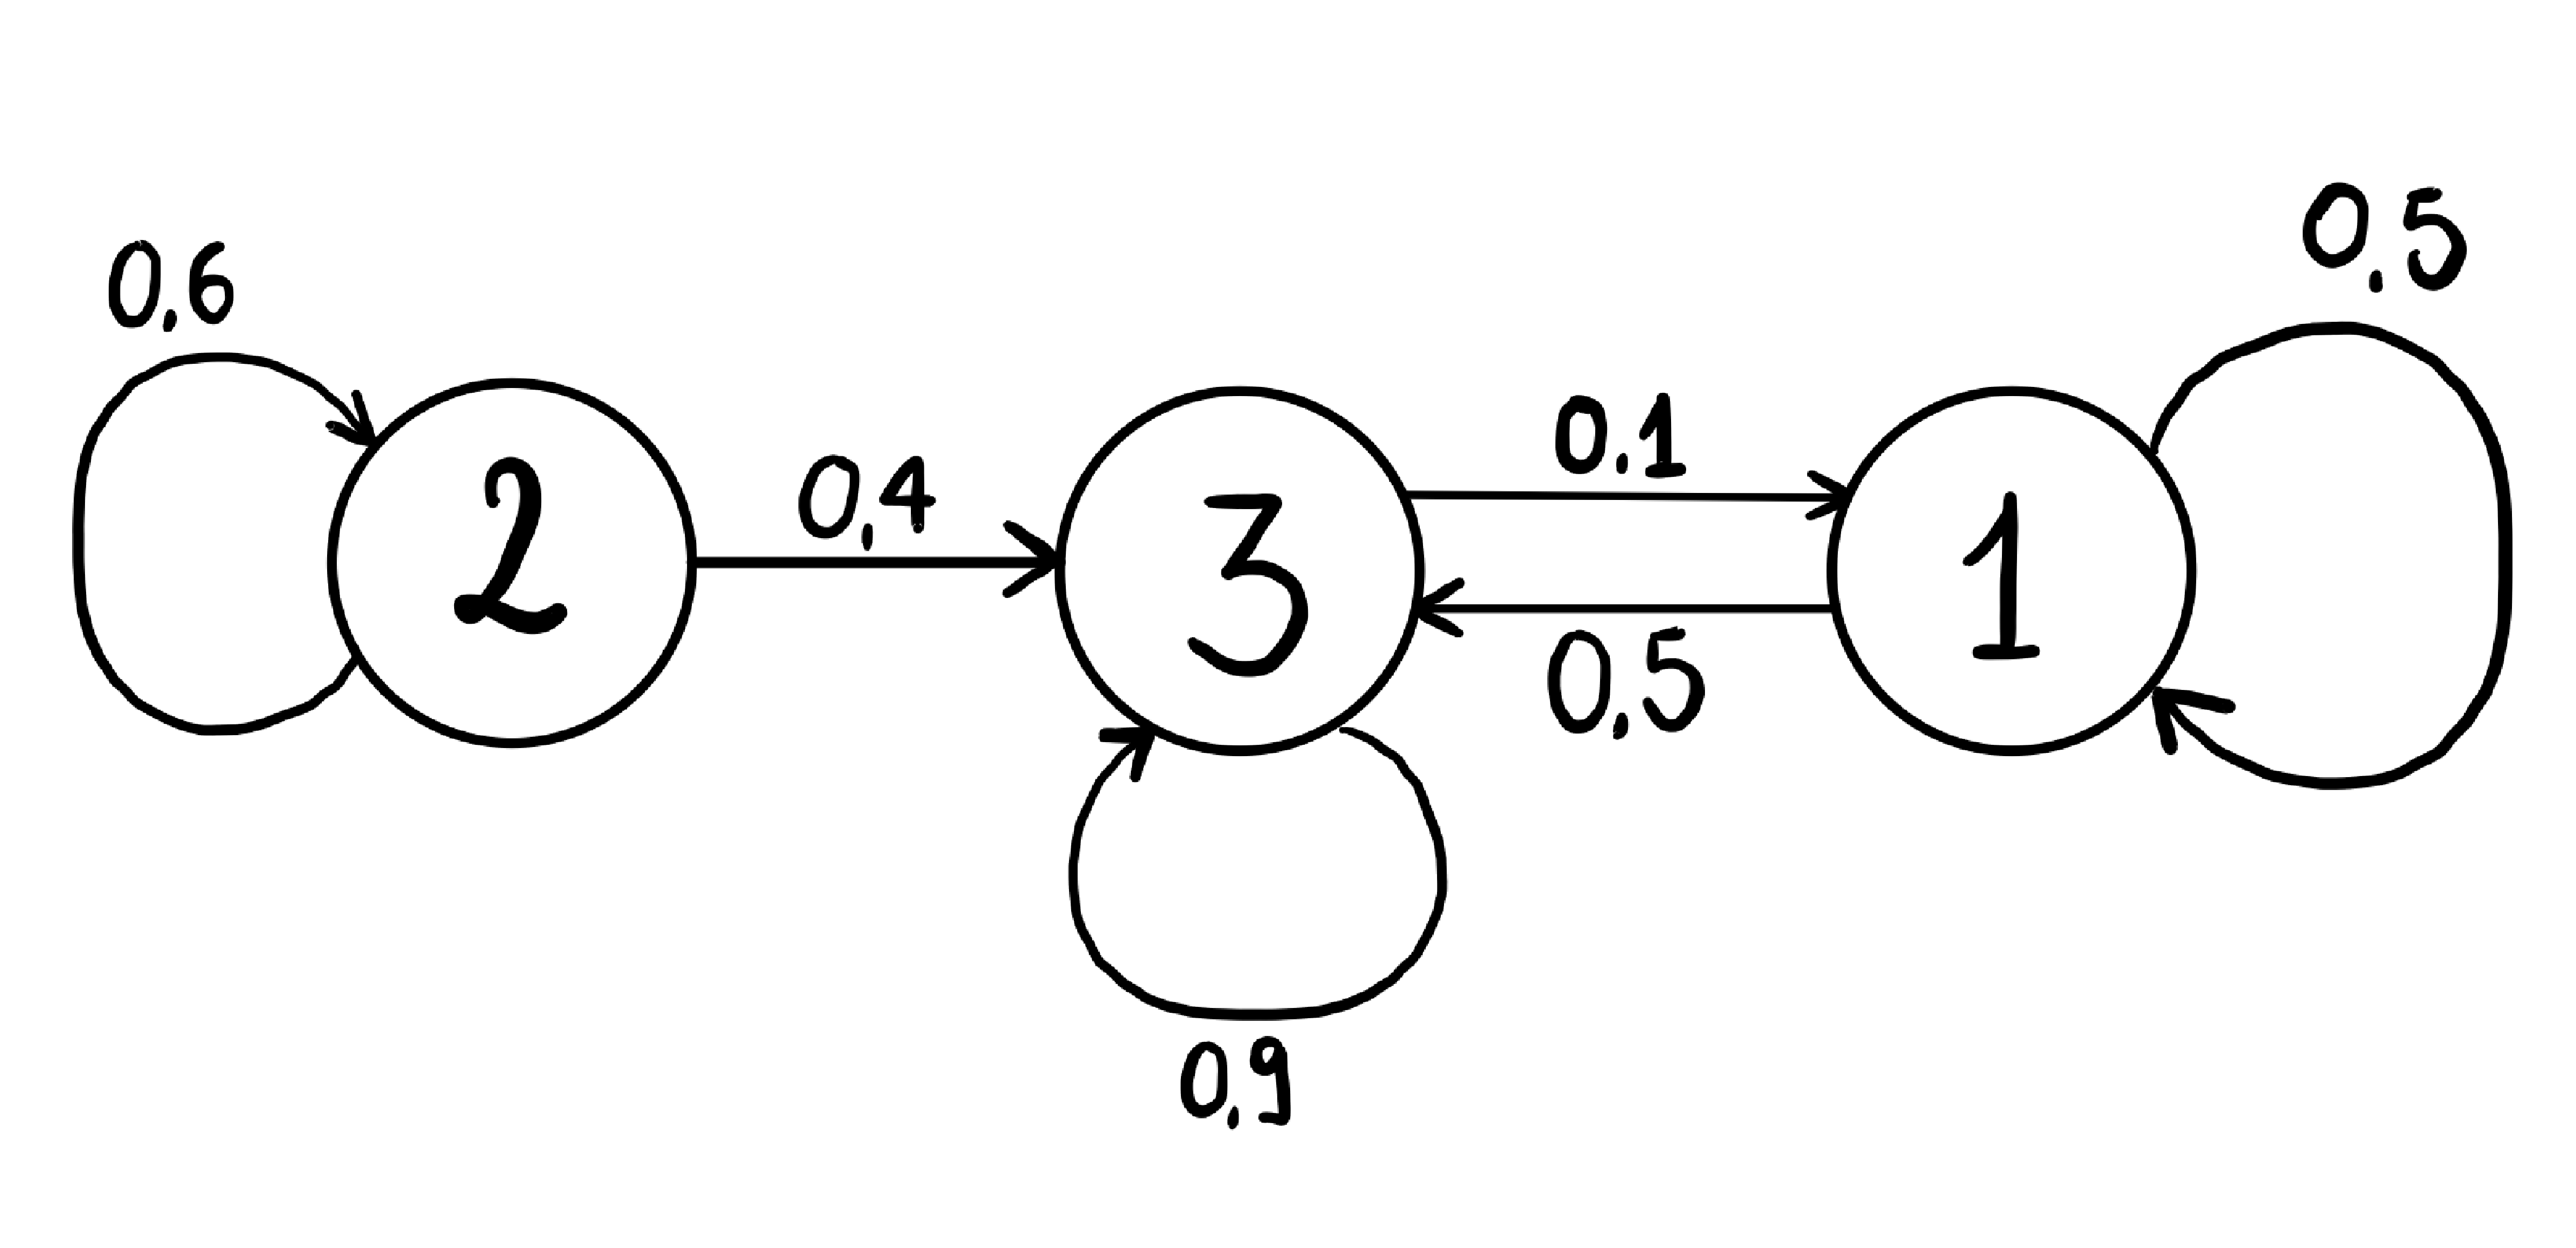
\includegraphics[scale=0.08]{Catena2.2.eps}
\captionof{figure}{Catena 2.}
  \end{figure}

  aventi matrici di transizione rispettivamente
  \begin{align*}
    P_{1}=\begin{bmatrix}
        0 & 0 & 1\\
        0.4 & 0.6 & 0\\ 
        0.2 & 0 & 0.8\\
      \end{bmatrix}, &&  
      P_{2}=\begin{bmatrix}
         0.5 & 0 & 0.5\\
         0 & 0.6 & 0.4\\
         0.1 & 0 & 0.9\\ 
      \end{bmatrix}.
    \end{align*}
 
  In entrambi i casi lo stato $\{2\}$ è transiente mentre $\{1,3\}$ è l'insieme dei ricorrenti. 
La distribuzione stazionaria sarà data da 
   \begin{align*}
   &\pi_1(1) = \frac{0.2}{1+0.2} && \pi_1(2) = 0 &&    \pi_1(3) = \frac{1}{1+0.2}\\
   &\pi_2(1) = \frac{0.1}{0.5+0.1} && \pi_2(2) = 0
 &&\pi_2(3) = \frac{0.5}{0.5+0.1} 
     \end{align*}
     e quindi pari a 
     \begin{equation*}
     \pi_{1,2} = \left(\frac{1}{6}, 0, \frac{5}{6}\right).
     \end{equation*}
     
Per poter calcolare la distribuzione limite delle due catene, invece, bisogna considerare le differenti possibili inizializzazioni. \\
\newpage
Per la catena 1 si ha: 
\begin{flushleft}
\begin{itemize}

\item
$\displaystyle\lim_{n \to \infty} \mathbb{P}(X_n=1 \lvert X_0 = j) = \pi(1) = \frac{1}{6};\) \quad\quad\quad con $j = 1,3;$\\
\item
$\displaystyle\lim_{n \to \infty} \mathbb{P}(X_n=1 \lvert X_0 = 2) = \lim_{n \to\infty} \mathbb{P}(X_n=1)\cdot \mathbb{P}(X_1=1 \lvert X_0 = 2)= 0.4\cdot\pi(1) = \frac{1}{15};$ 
\item
$\displaystyle\lim_{n \to \infty} \mathbb{P}(X_n=2 \lvert X_0= x) = \lim_{n \to \infty} \mathbb{P}(X_n = 2) = 0;$\\
\item
$\displaystyle\lim_{n \to \infty} \mathbb{P}(X_n=3 \lvert X_0 = j) = \pi(3) = \frac{5}{6};$ \quad\quad\quad con $j = 1,3;$\\
\item
$\displaystyle\lim_{n \to \infty} \mathbb{P}(X_n=3 \lvert X_0 = 2) =  0.4\cdot\pi(3) = \frac{1}{3};$ 
\end{itemize}
\end{flushleft}

Allo stesso modo per la catena 2 si verifica: 
\begin{flushleft}
\begin{itemize}
\item
$\displaystyle\lim_{n \to \infty} \mathbb{P}(X_n=1 \lvert X_0 = j) = \pi(1) = \frac{1}{6};\) \quad\quad\quad con $j = 1,3;$\\
\item
$\displaystyle\lim_{n \to \infty} \mathbb{P}(X_n=1 \lvert X_0 = 2) = \lim_{n \to\infty} \mathbb{P}(X_n=1 \lvert X_1 = 3)\cdot \mathbb{P}(X_1=3 \lvert X_0 = 2)= 0.4\cdot\pi(1) = \frac{1}{15};$ 
\item
$\displaystyle\lim_{n \to \infty} \mathbb{P}(X_n=2 \lvert X_0= x) = \lim_{n \to \infty} \mathbb{P}(X_n = 2) = 0;$\\
\item
$\displaystyle\lim_{n \to \infty} \mathbb{P}(X_n=3 \lvert X_0 = j) = \pi(3) = \frac{5}{6};$ \quad\quad\quad con $j = 1,3;$\\
\item
$\displaystyle\lim_{n \to \infty} \mathbb{P}(X_n=3 \lvert X_0 = 2) =  0.4\cdot\pi(3) = \frac{1}{3};$ 
\end{itemize}
\end{flushleft}
In ambo i casi ottiene quindi che se le DTMC sono inizializzate a $X_0 = 2$ la distribuzione limite è
  \begin{equation*}
  \left(\frac{1}{15}, 0, \frac{1}{3}\right)',
  \end{equation*}
  altrimenti per $X_0 = 1, X_0 = 3$ si ha 
  \begin{equation*}
  \left(\frac{1}{6}, 0, \frac{5}{6}\right)'.
  \end{equation*}

  \newpage
  \item
  
  Due DTMC a stati finiti, diverse, non irriducibili, che ammettono la stessa famiglia di distribuzioni stazionarie, potrebbero essere le seguenti. 
 \begin{figure}[htb]\centering

\includegraphics[scale=0.09]{Catena3.1.eps}
\captionof{figure}{Catena 1.}
  \end{figure}
  \begin{figure}[h]\centering
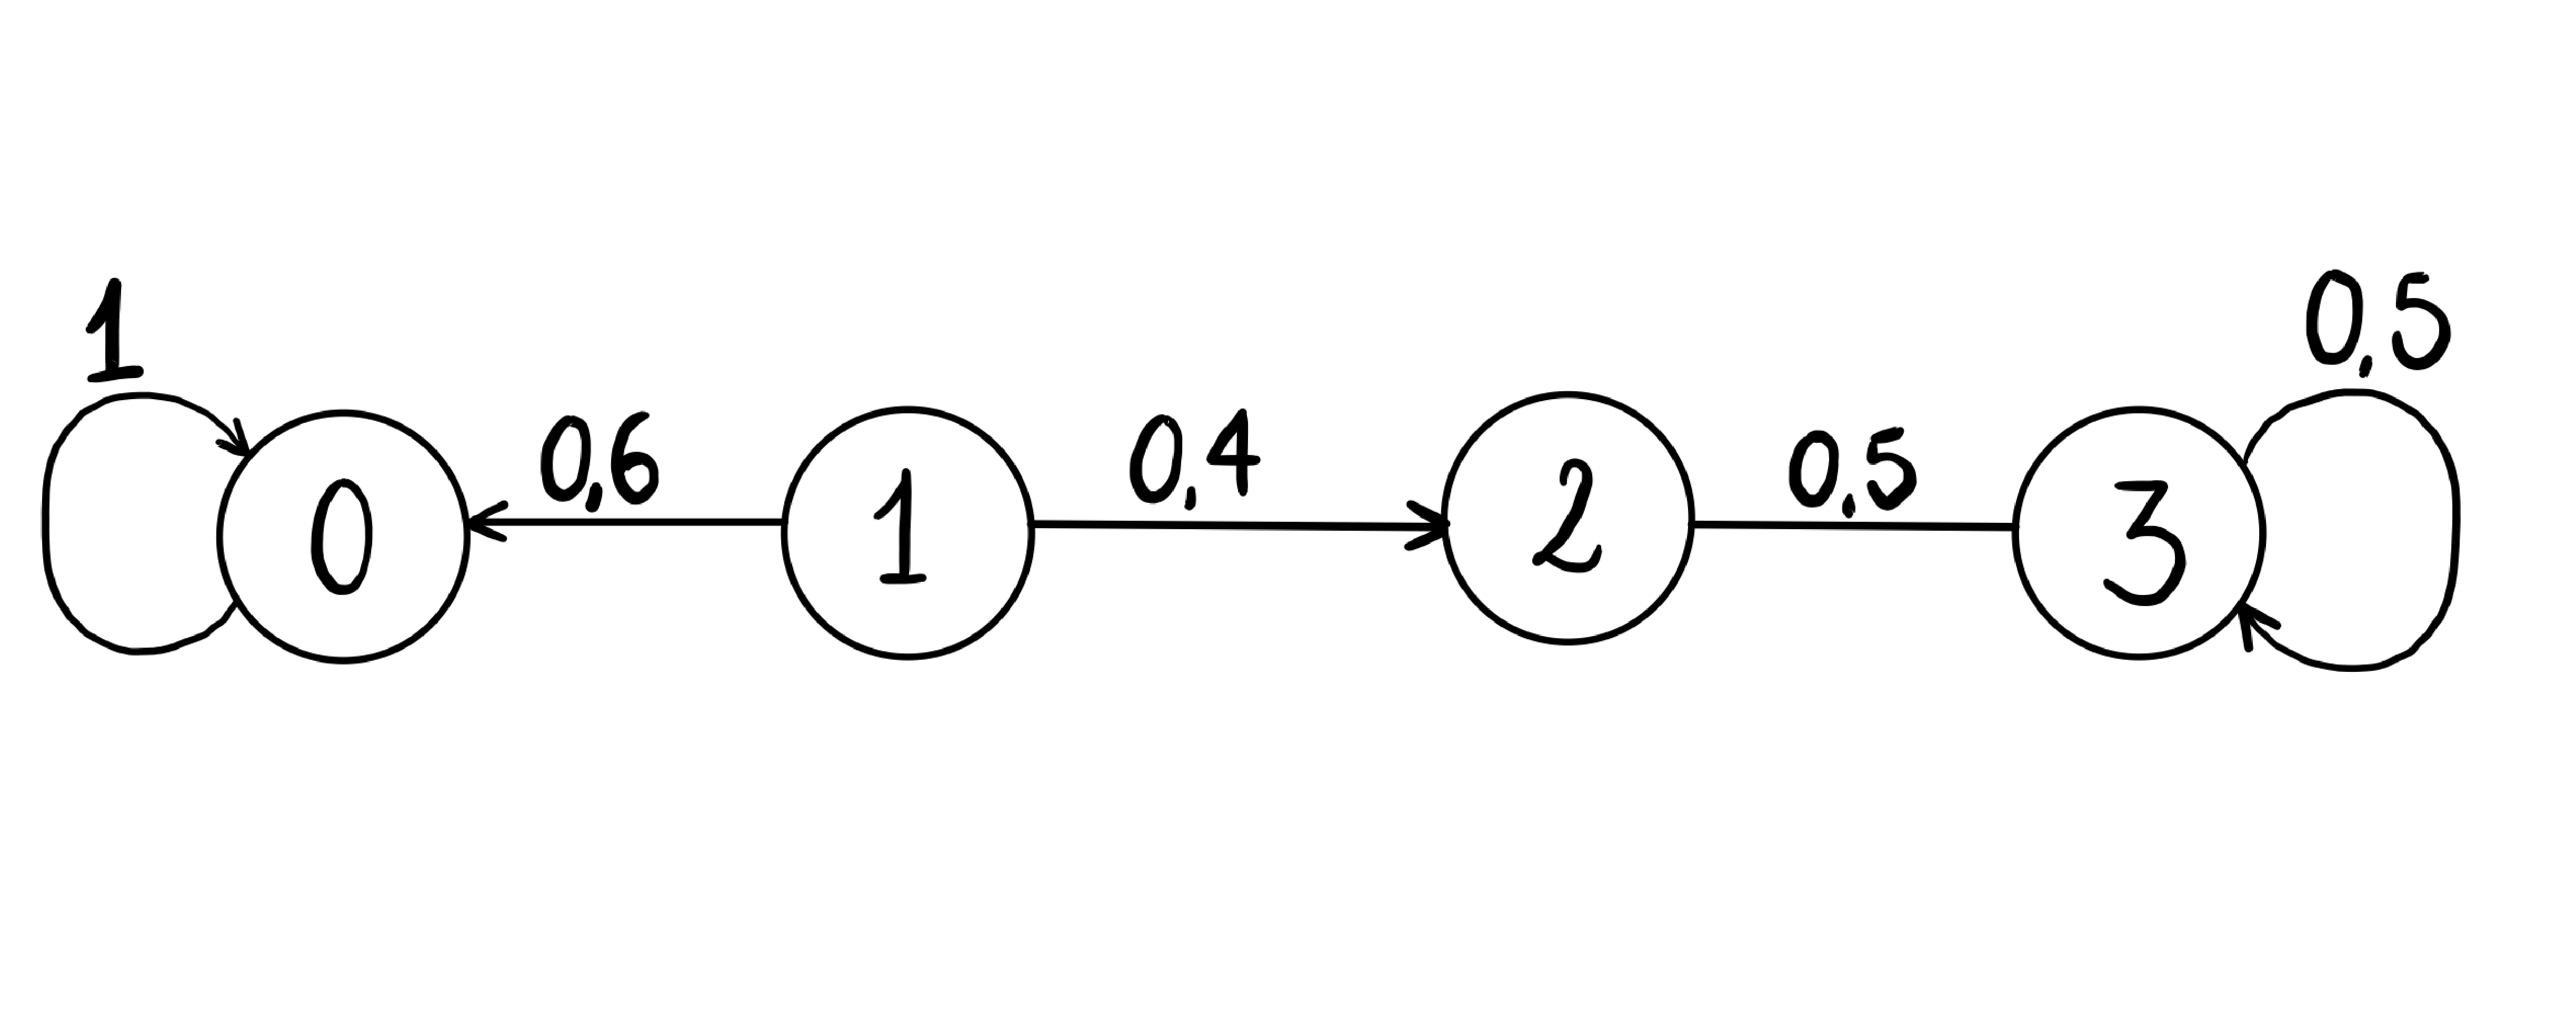
\includegraphics[scale=0.11]{Catena3.2.eps}
\captionof{figure}{Catena 2.}
  \end{figure}
     
  La matrice di trasizione $P_1$ vale 
  \[\begin{bmatrix}
        1 & 0 & 0 & 0\\
        0.3 & 0 & 0.6 & 0.1\\ 
        0 & 0 & 0.5 & 0.5\\
        0 & 0 & 0.5 & 0.5\\
      \end{bmatrix}\]
La catena non è irriducibile. Vi è uno stato transiente, $T = \{1\}$ mentre gli insiemi ricorrenti sono $R_1 = \{0\}$ e $R_2 = \{2,3\}$. Questo implica che le distribuzioni seguenti siano entrambe stazionarie 
\begin{align*}
\pi_1 = (1, 0, 0, 0)\,\,\,\,\,\,e\,\,\,\,\,\, \pi_2= (0, 0, \frac{1}{2}, \frac{1}{2}) 
\end{align*}
e che appartengano alla famiglia di distribuzioni data da 
\[(\alpha_1, 0, \frac{\alpha_2}{2}, \frac{\alpha_2}{2})\]
dove $\alpha_1, \alpha_2 \geq 0$, con $\alpha_1+\alpha_2 = 1$.


La catena 2 invece ha matrice di transizione $P_2$ 
  \[\begin{bmatrix}
        1 & 0 & 0 & 0\\
        0.6 & 0 & 0.4 & 0\\ 
        0 & 0 & 0.5 & 0.5\\
        0 & 0 & 0.5 & 0.5\\
      \end{bmatrix}\]

Anche in questo caso la DTMC ha due set di stati  ricorrenti $R_1 = \{0\}$ e $R_2 = \{2,3\}$ per i quali si possono trovare almeno due distribuzioni stazionarie differenti, quali
\begin{align*}
\pi_1 = (1, 0, 0, 0)\,\,\,\,\,\,e\,\,\,\,\,\, \pi_2= (0, 0, \frac{1}{2}, \frac{1}{2}).
\end{align*}
Dati $\beta_1, \beta_2 \geq 0$, con $\beta_1+\beta_2 = 1$, tutte le distribuzioni di $P_2$ sono del tipo 
\[(\beta_1, 0, \frac{\beta_2}{2}, \frac{\beta_2}{2}),\]identiche a $P_1$. 
  
     
\newpage
\item
Utilizzando le catene del punto precedente, ne calcoliamo la distribuzione al limite per tutte le possibili inizializzazioni della catena. Per la catena 1 si avrà: 

\begin{itemize}
\item
$\mathbb{P}(X_n = 1)$, per $n \rightarrow \infty$: 
\[ \lim_{n \to \infty} \mathbb{P}(X_n= 1 \lvert X_0 = x) = 0, \quad\quad x \in \{0,1,2,3\}. \]
\item
$\mathbb{P}(X_n = 0)$, per $n \rightarrow \infty$: 
\[\lim_{n \to \infty} \mathbb{P}(X_n=0 \lvert X_0 = 0) = 1;\]
\begin{multline*}
\lim_{n \to \infty} \mathbb{P}(X_n=0 \lvert X_0 = 1)= \lim_{n \to \infty} \mathbb{P}(X_n=0 \lvert X_1 = 0)\cdot\mathbb{P}(X_1=0 \lvert X_0 = 1)\\
= 0.3\cdot \pi_1(0) = \frac{3}{10};
\end{multline*} 
\[\lim_{n \to \infty} \mathbb{P}(X_n=0 \lvert X_0= x) = 0, \quad\quad x \in \{2,3\}. \]

%per Xn = 2 
\item
$\mathbb{P}(X_n = 2)$, per $n \rightarrow \infty$: 
\[\lim_{n \to \infty} \mathbb{P}(X_n=2 \lvert X_0 = 0) = 0;\] 
\begin{multline*} 
\lim_{n \to \infty} \mathbb{P}(X_n=2 \lvert X_0 = 1)=\lim_{n \to \infty} \mathbb{P}(X_n=2 \lvert X_1 = 2)\cdot\mathbb{P}(X_1=2 \lvert X_0 = 1) +\\
+\lim_{n \to \infty} \mathbb{P}(X_n=2 \lvert X_1 = 3)\cdot\mathbb{P}(X_1=3 \lvert X_0 = 1) = 0.6\cdot \pi_2(2) + 0.1\cdot \pi_2(2)  = \frac{7}{20};
\end{multline*}
\[\lim_{n \to \infty} \mathbb{P}(X_n=2 \lvert X_0= x) = \pi_2(2) = \frac{1}{2}, \quad\quad x \in \{2,3\}.\]
\item
$\mathbb{P}(X_n = 1)$, per $n \rightarrow \infty$: 
\[\lim_{n \to \infty} \mathbb{P}(X_n=3 \lvert X_0 = 0) = 0;\] 
\begin{multline*}
\lim_{n \to \infty} \mathbb{P}(X_n=3 \lvert X_0 = 1)=\lim_{n \to \infty} \mathbb{P}(X_n=3 \lvert X_1 = 3)\cdot\mathbb{P}(X_1=3 \lvert X_0 = 1) +\\
+\lim_{n \to \infty} \mathbb{P}(X_n=3 \lvert X_1 = 2)\cdot\mathbb{P}(X_1=2 \lvert X_0 = 1) = 0.1\cdot \pi_2(3) + 0.6\cdot \pi_2(3)  = \frac{7}{20};
\end{multline*}
\[\lim_{n \to \infty} \mathbb{P}(X_n=3 \lvert X_0= x) = \pi_2(3) = \frac{1}{2},\quad\quad x \in \{2,3\}. \]
\end{itemize}

Il motivo per cui la distribuzione al limite non è unica risiede nella non irriducibilità della catena. Si avrà pertanto che:
\begin{itemize}
\item
se $X_0 = 0$ la distribuzione limite corrisponde alla distribuzione stazionaria dove $\alpha_1 = 1$ e $\alpha_2 = 0$
\[(1,0,0,0)\]
\item
se $X_0 = 1$ la distribuzione limite è quella in cui $\alpha_1 = 0.3$ e $\alpha_2 = 0.7$
\[\left(\frac{3}{10},0,\frac{7}{20},\frac{7}{20}\right)\]
\item
se $X_0 = 2$ oppure $X_0 = 3$ i due coefficienti valgono $\alpha_1 = 0$ e $\alpha_2 = 1$
\[\left(0,0,\frac{1}{2},\frac{1}{2}\right).\]

\end{itemize}


\subsection* {}
Allo stesso modo si calcolano le distribuzioni limite per la seconda DTMC. Si ottengono i risultati seguenti: 
\begin{itemize}
\item
se $X_0 = 0$ si ha $\beta_1 = 1$ e $\beta_2 = 0$
\[\left(1,0,0,0\right)\]
\item
se $X_0 = 1$ la distribuzione limite è quella in cui $\beta_1 = 0.6$ e $\beta_2 = 0.2$
\[\left(\frac{3}{5},0,\frac{1}{5},\frac{1}{5}\right)\]
\item
se $X_0 = 2$ oppure $X_0 = 3$ i due coefficienti valgono $\beta_1 = 0$ e $\beta_2 = 1$
\[\left(0,0,\frac{1}{2},\frac{1}{2}\right).\]
\end{itemize}

  \newpage
  \item
  Una DTCM a stati infiniti che ammette distribuzione stazionaria potrebbe essere la seguente:
  
  \begin{figure}[htb]\centering
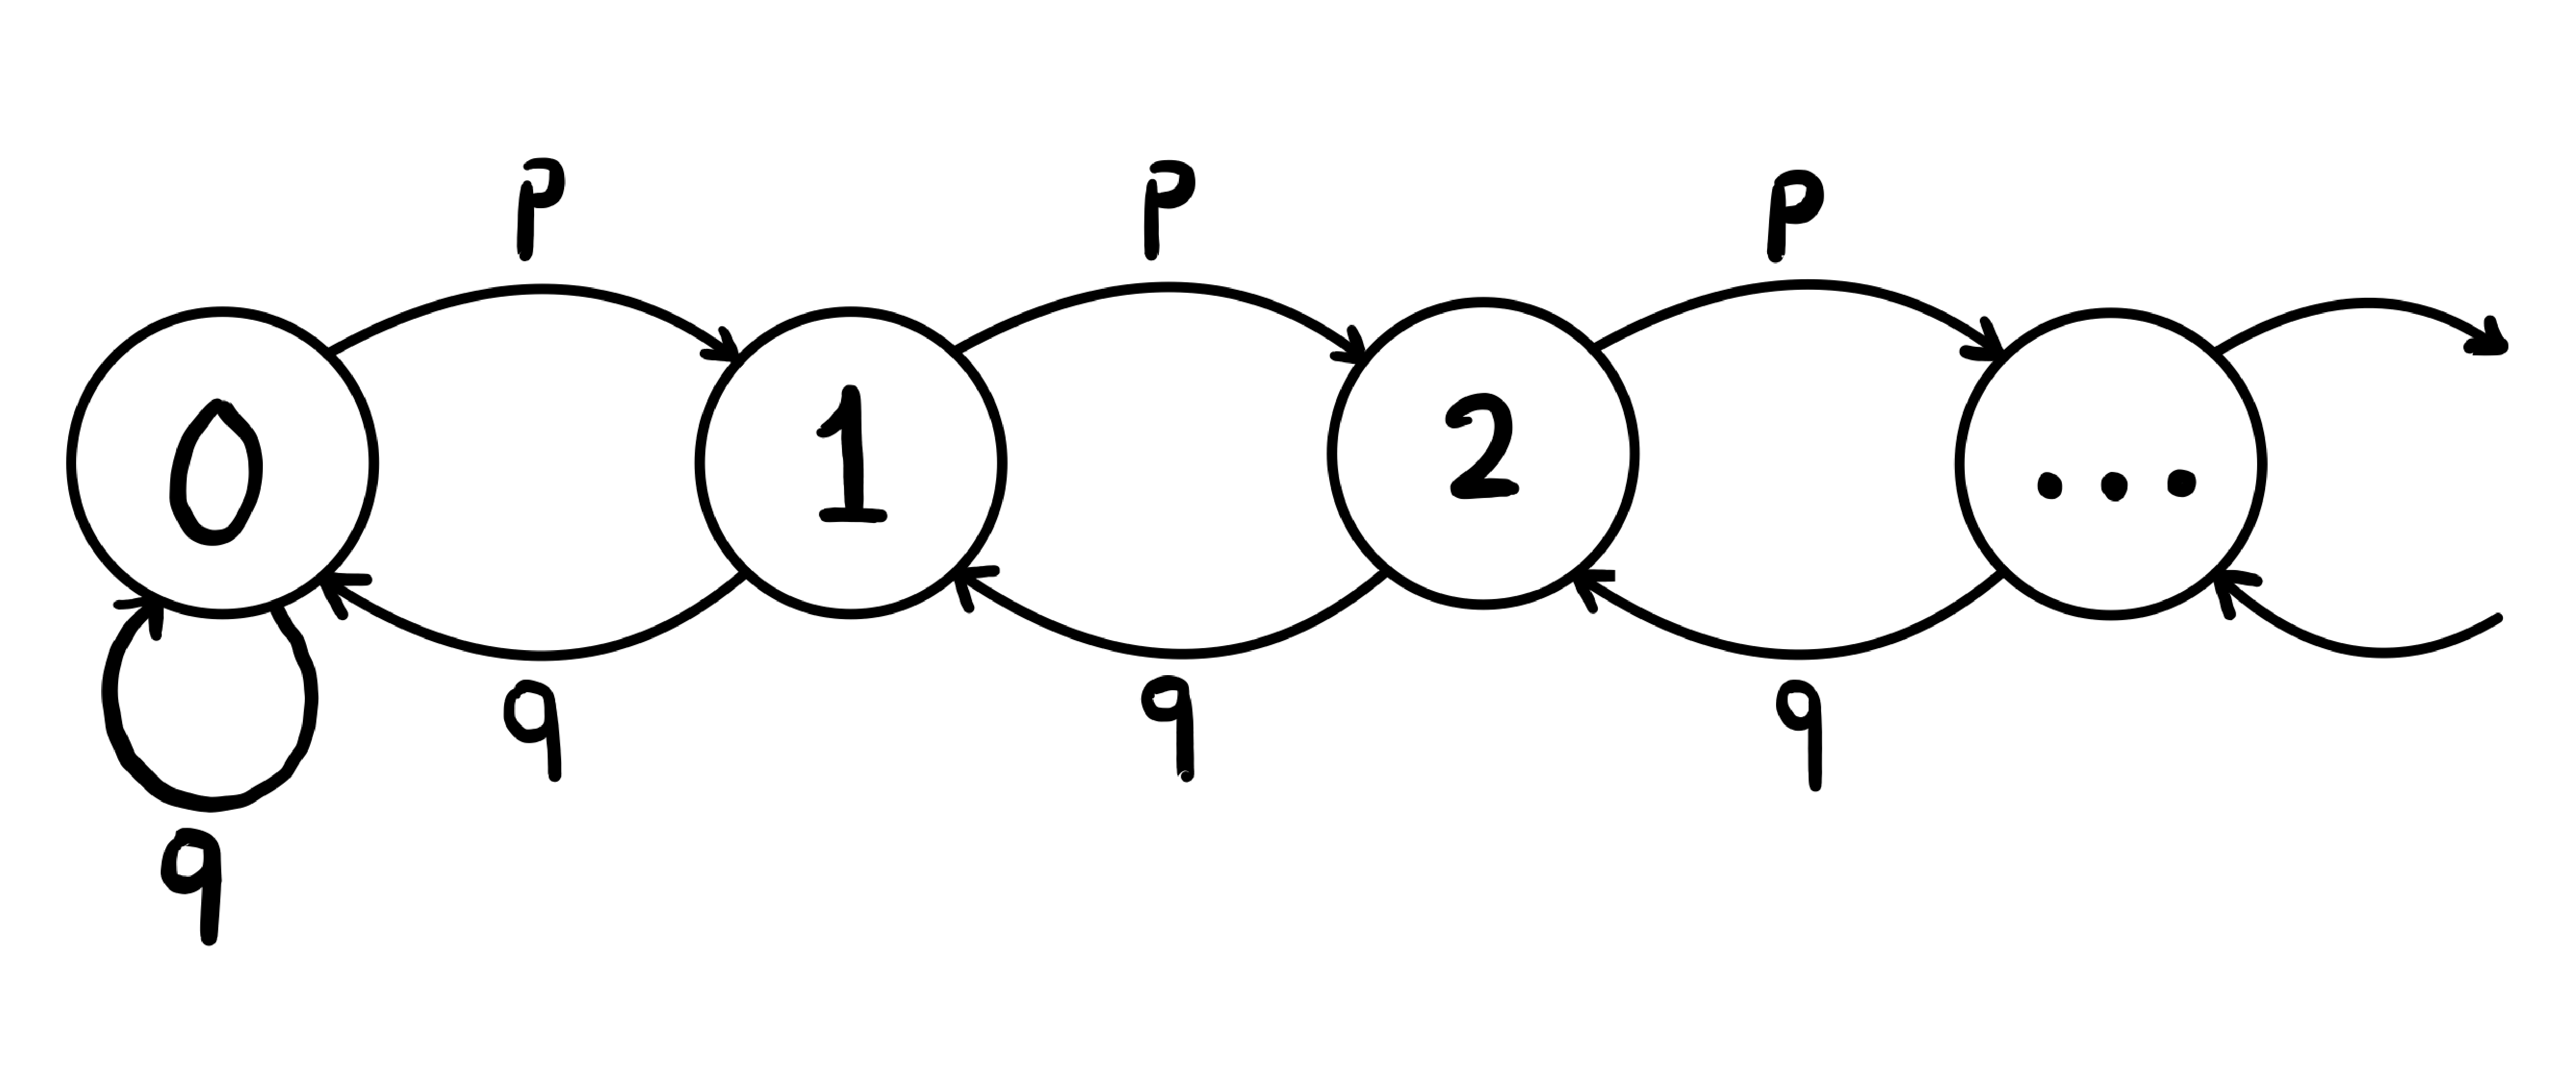
\includegraphics[scale=0.1]{Catena5.1}
  \end{figure}
  
  Questa è una catena di nascita e morte sui numeri naturali, incluso lo 0. Sappiamo che, per le catene di questo tipo la distribuzione stazionaria esiste sotto determinate condizioni. In particolare ogni catena di nascita è morte ha un'unica distribuzione stazionaria se e solo se 
  \begin{align*}
  0 <  \sum_{x=0}^{\infty}\prod_{i=0}^{x-1}\frac{p_i}{q_{i+1}} < \infty.
\end{align*}  
Ci basterà pertanto scegliere come esempio il cosiddetto ``1d partially reflected Random Walk'' a cui assegnamo le probabilità di transizione:
\begin{align*}
&p\left(x,x+1\right)=p_{x}=p = \frac{1}{3}, \,\,\, \forall x\geq0; \\
&p\left(x,x-1\right)=q_{x}=1-p= q = \frac{2}{3}, \,\,\, \forall x \geq 1; \\ 
&p\left(0,0\right)=1-p=q.
\end{align*}  
Per tale catena risulta che
\begin{equation*}
\sum_{x=0}^{\infty}\prod_{i=0}^{x-1}=\sum_{x=0}^{\infty}\prod_{i=0}^{x-1}\frac{p}{q}=\sum_{x=0}^{\infty}\left(\frac{p}{q}\right)^{x}
\end{equation*}
e questa serie converge a un numero finito se e solo se $p < \frac{1}{2}$. Solo in questo modo, infatti, si garantisce l'esistenza di una distribuzione stazionaria che nel nostro caso sarà pari a :
\begin{equation*}
\pi\left(x\right)=\left(1-\frac{p}{q}\right)\left(\frac{p}{q}\right)^{x} = \left(\frac{1}{2}\right)\cdot\left(\frac{1}{2}\right)^{x}=\left(\frac{1}{2}\right)^{x+1}
\end{equation*}
per ogni $x \in \mathbb{N}$ perchè tutti gli stati della catena sono positivo ricorrenti. 
\newpage
\item

Similmente al caso precedente, consideriamo ora  la catena di Markov a stati infiniti denominata ``1d Random Walk'' o ``cammino dell'ubriaco'', sullo spazio degli stati discreto $S=\mathbb{Z}=\{...-2,-1,0,1,2,...\}$ con probabilità di transizione: 
\begin{align*}
&p\left(i,i+1\right)=p;\\
&p\left(i,i-1\right)=q, \,\,\, con \,\,\, q = 1-p, \,\,\, \forall i\in \mathbb{Z}.
\end{align*}
Osserviamo che se $p \neq \frac{1}{2}$ tutti gli stati sono transienti e quindi non esiste una distribuzione stazionaria.
Se invece $p = q = \frac{1}{2}$, nonostante la catena sia irriducibile e ricorrente e pertanto garantisce l'esistenza di una misura stazionaria $\eta(x)$, non è possibile trovare una distribuzione stazionaria perché bisognerebbe assicurare che 
\[\sum_{x \in \mathbb{Z}} \pi(x) = 1\] 
il che è impossibile. 
%\begin{figure}[htb]\centering
%\includegraphics[scale=0.4]{catenaex1_6.jpg}
  %\end{figure}
 
\end{enumerate}

  \newpage
\section{}%---------------ESERCIZIO 2 2-----------------------------------   

Supponiamo che una catena di Markov sia fatta da un insieme di stati ricorrenti $R$ e da uno transiente $T$, come nell'esempio.
\\Uno stato $y$ è ricorrente se e solo se 
\begin{gather*}
  \mathbb{E}_y(N(y)) =  \sum \limits_{n=1}^{\infty} p^{(n)}(y,y) = \infty
\end{gather*}
Inoltre, la ricorrenza è una proprietà di classe quindi tutti gli stati comunicanti con \(y\) sono ricorrenti.
\\
Sia \(x\) un generico stato transiente e \(y\) uno stato ricorrente in cui è inizializzata la catena. Sia per assurdo \(p^{(k)}(y,x)>0\) per qualche \(k\) intero, ossia supponiamo per assurdo che, partendo da uno stato ricorrente, la catena possa visitare al tempo \(k\) uno stato transiente. Andiamo a valutare la quantità \(p^{(n)}(j,j)\) ossia la probabilità di ritorno in \(x\). Dal teorema di Chapman-Kolmogorov si ottiene:
\begin{gather*}
  p^{(m+n+k)}(x,x) \geq p^{(m)}(x,y)p^{(n)}(y,y)p^{(k)}(y,x)
\end{gather*}
Pertanto\begin{gather*}
  \mathbb{E}_x(N(x)) =  \sum \limits_{n=1}^{\infty} p^{(n)}(x,x) \geq \sum \limits_{n=1}^{\infty} p^{(n+m+k)}(x,x) \\
  \geq p^{(m)}(x,y)p^{(k)}(y,x)\sum \limits_{n=1}^{\infty} p^{(n)}(y,y) = \infty
\end{gather*}
Quindi lo stato \(x\) risulterebbe essere anch'esso ricorrente, arrivando ad un assurdo.

\newpage

\section{}%---------------ESERCIZIO 3 ------------------------------------------
Il problema si presenta in una forma in cui, partendo da uno stato \(x\), il numero di passi per arrivare nello stato \(n\) è pari al numero di passi per uscire dalla zona tegli stati transienti. Per come è definito il problema i nodi da \(1\) a \(n-1\) sono gli stati transienti della catena e pertanto appartengono all'insieme \(T\) mentre l'unico stato ricorrente (pertanto assorbente) è rappresentato dal nodo \(n\) che sarà l'unico elemento dell'insieme \(R\). \\
Quella cercata è pertanto l'attesa del numero di passi per arrivare da uno stato \(T\) ad uno stato \(R\), ossia un \textit{expected exit time}:
\begin{gather*}
  m_x = \mathbb{E}_x \left[ \sum \limits_{n=0}^{\infty} \mathbbm{1}_{\{X_n \notin R\}}\right] = (Qe)_x
\end{gather*}
Dove \(Q \in \mathbb{R}^{\#T \times \#T}\) è la matrice delle visite attese ad uno stato transiente. In particolare:
\begin{gather*}
  Q = (I-P_{T,T})^{-1} \Rightarrow (I-P_{T,T})m = e
\end{gather*}
Dove \(I-P_{T,T}\) è una matrice triangolare superiore, pertanto il sistema può essere risolto per sostituzione.
\begin{gather*}
  \begin{bmatrix}
    1 & -\frac{1}{n-1} & -\frac{1}{n-1} & \dots & -\frac{1}{n-1} \\
    0 & 1 & -\frac{1}{n-2} & \dots & -\frac{1}{n-2} \\
    \vdots & & \ddots & & \\
    0 &\dots & & 1 & -\frac{1}{n-(n-2)}\\
    0 &\dots  & & & 1
  \end{bmatrix}
  \begin{bmatrix}
    m_1 \\ m_2 \\ \vdots \\ m_{n-2} \\ m_{n-1}
  \end{bmatrix}=
  \begin{bmatrix}
    1 \\ 1 \\ \vdots \\ 1 \\ 1
  \end{bmatrix}
\end{gather*}
Il sistema può essere risolto per induzione con soluzione:
\begin{gather} \label{eq:mni}
  m_{n-i} =  \sum \limits_{k=1}^{i} \frac{1}{n-(n-k)} =  \sum \limits_{k=1}^{i} \frac{1}{k}
\end{gather}
infatti abbiamo:
\begin{gather*}
m_{n-1} = 1\\
m_{n-2}=1+\frac{1}{2}=\sum_{k=1}^{2}\frac{1}{k}.
\end{gather*} 
Supponendo quindi vero il predicato per i valori \(\{i-1, i-2, \dots , 1\}\) andiamo a dimostrare \ref{eq:mni} utilizzando la forma del sistema triangolare superiore:
\begin{gather*}
  m_{n-i} = 1 + \frac{1}{i}\left( \sum \limits_{k=1}^{i-1}\frac{1}{k} + \sum \limits_{k=1}^{i-2}\frac{1}{k} + \sum \limits_{k=1}^{i-3}\frac{1}{k} + \dots + \sum \limits_{k=1}^{1}\frac{1}{k} \right) = \\
  1 + \frac{1}{i}\left(\sum \limits_{k=1}^{i-1}\frac{1}{k}(i-k)\right) = 1 + \frac{1}{i}\left( \left(\sum \limits_{k=1}^{i-1}\frac{i}{k}\right)- (i-1)\right) = \\
   \frac{1}{i} +\sum \limits_{k=1}^{i-1}\frac{1}{k} = \sum \limits_{k=1}^{i}\frac{1}{k}.
\end{gather*}
È inoltre possibile scrivere gli elementi del vettore \(m\) nella seguente forma:
\begin{gather*}
  m_j = \sum \limits_{k=1}^{n-j}\frac{1}{k}
\end{gather*}
pertanto 
\begin{gather*}
  \lim \limits_{n \rightarrow \infty} m_j = \lim \limits_{n \rightarrow \infty} \sum \limits_{k=1}^{n-j}\frac{1}{k} = \infty \,,\,\,\, \forall j \text{ fissato}
\end{gather*}





\newpage
\section{}%---------------ESERCIZIO 4 ------------------------------------------
 \begin{figure}[htb]\centering
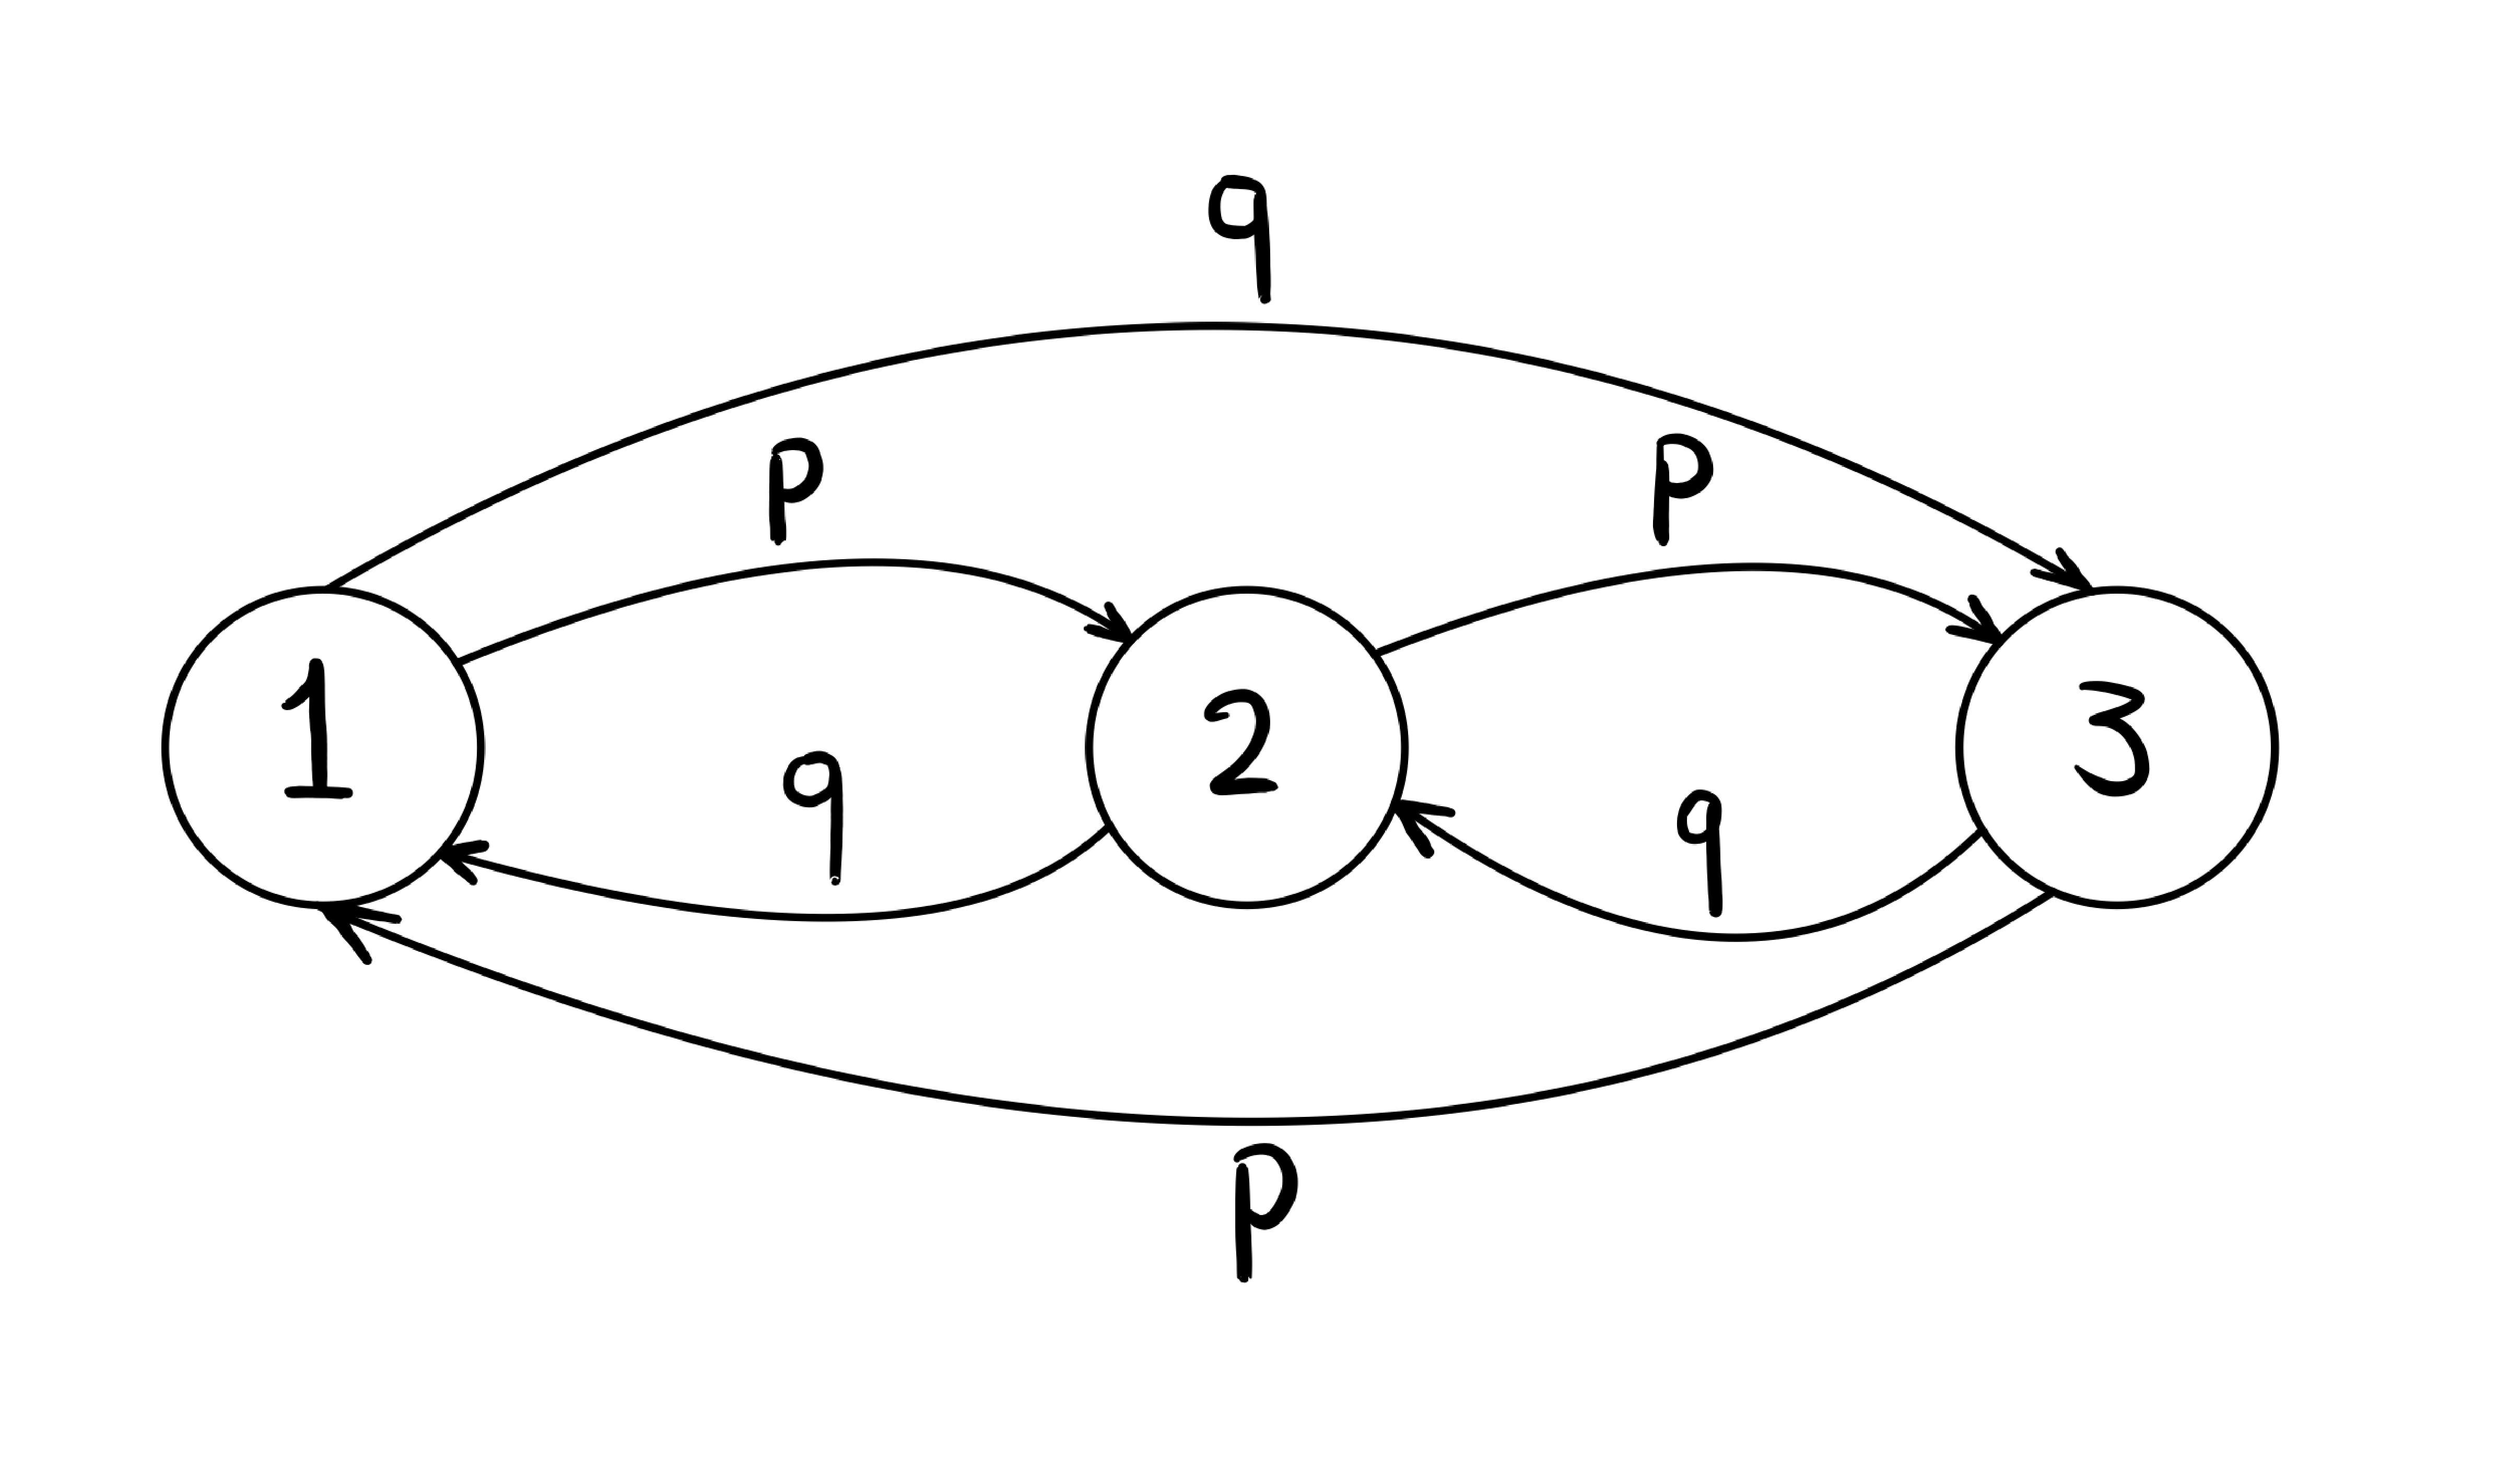
\includegraphics[scale=0.09]{Catena4.eps}
  \end{figure}
  Sappiamo che una distribuzione di bilancio dettagliato, se esiste, è anche una distribuzione stazionaria.\\
  Consideriamo allora il sistema relativo all'esistenza di una distribuzione di bilancio dettagliato nel caso della catena di Markov in questione:
  \begin{equation*}
  \begin{cases}\pi_{1}p=\pi_{2}\left(1-p\right)\\\pi_{1}\left(1-p\right)=\pi_{3}p\\\pi_{2}p=\pi_{3}\left(1-p\right)\end{cases}\Leftrightarrow\begin{cases}\pi_{1}p-\pi_{2}\left(1-p\right)=0\\\pi_{1}\left(1-p\right)-\pi_{3}p=0\\\pi_{2}p-\pi_{3}\left(1-p\right)=0\end{cases}.
  \end{equation*}
  Studiando il rango della matrice
  \begin{equation*}
  A=\begin{bmatrix}
  p & p-1 & 0\\
  1-p & 0 & -p \\
  0 & p & p-1\\
  \end{bmatrix},
  \end{equation*}
 si ricava che
 \begin{gather*}
 \det A=p^{3}+\left(p-1\right)^{3}=0\Leftrightarrow p^{3}=\left(1-p\right)^{3}\Leftrightarrow p=1-p.
 \end{gather*}
 Allora, se $p\neq \left(1-p\right)$, il sistema ammette solo la soluzione banale che, però, non identificando una distribuzione, non può essere accettata.\\
 Se $p=\left(1-p\right)$, invece, il rango di $A$ è $2$ e, dunque, il sistema ammette la soluzione non banale $\pi_{1}=\pi_{2}=\pi_{3}$ che, imponendo la condizione $\pi_{1}+\pi_{2}+\pi_{3}=1$, si traduce in $\pi\equiv\left(\frac{1}{3},\frac{1}{3},\frac{1}{3}\right)'$.\\
 Quindi, nell'ultimo caso, abbiamo trovato anche una distribuzione stazionaria, che è quella tale per cui $p=\frac{1}{2}$ e $\pi\equiv\left(\frac{1}{3},\frac{1}{3},\frac{1}{3}\right)'$.
 
 \newpage
\section{}%---------------ESERCIZIO 5 ------------------------------------------ 
\begin{enumerate}
\item[(1)]
  I processi $N_{1}\left(t\right)$ e $N_{2}\left(t\right)$ possono essere scritti come
  \begin{align*}
  N_{1}\left(t\right)=N\left(\int_{0}^{t}\lambda_{1}\left(u\right) \,du\right) \,\,\, \text{e} \,\,\, N_{2}\left(t\right)=N\left(\int_{0}^{t}\lambda_{2}\left(u\right) \,du \right),
  \end{align*}
  dove $N\left(t\right)$ è un processo di Poisson di rate $1$ (per il teorema del ``riscalamento'' del tempo di un processo di Poisson di rate $1$).\\
  Adesso, possiamo applicare la proprietà di ``supercondition'' per processi di Poisson non omogenei, la quale afferma che se abbiamo $N_{1}\left(t\right),...,N_{k}\left(t\right)$ processi di Poisson indipendenti di rates, rispettivamente, $\lambda_{1}\left(t\right),...,\lambda_{k}\left(t\right)$, allora $N_{1}\left(t\right)+...+N_{k}\left(t\right)$ è un processo di Poisson di rate $\lambda_{1}\left(t\right)+...+\lambda_{k}\left(t\right)$.\\
  Nel nostro caso, allora,
  \begin{equation*}
  N_{1}\left(t\right)+N_{2}\left(t\right)= N\left(\int_{0}^{t}\lambda_{1}\left(u\right) \,du\right) + N\left(\int_{0}^{t}\lambda_{2}\left(u\right) \,du \right)
  \end{equation*}
  è un processo di Poisson non omogeneo di rate $\lambda_{1}\left(t\right)+\lambda_{2}\left(t\right)$.\\
  \item[(2)]
  Il processo $D\left(t\right)=N_{1}\left(t\right)-N_{2}\left(t\right)$ non è più un processo di Poisson non omogeneo.\\
  Infatti, ponendo
  \begin{equation*}
  D\left(t\right)=N\left(\int_{0}^{t}\lambda_{1}\left(u\right) \,du\right) - N\left(\int_{0}^{t}\lambda_{2}\left(u\right) \,du \right),
  \end{equation*}
   con $N\left(t\right)$ processo di Poisson di rate 1, come in precedenza, risulta che, $\forall t,s$, con $s<t$, risulta che $D\left(t\right)-D\left(s\right)$ segue una distribuzione di Skellam di parametri $\left(\int_{s}^{t}\lambda_{1}\left(u\right) \,du,\int_{s}^{t}\lambda_{2}\left(u\right) \,du \right)$.\\
   Infatti
   \begin{align*}
   &D\left(t\right)-D\left(s\right)=  N_{1}\left(t\right)-N_{2}\left(t\right)-N_{1}\left(s\right)+N_{2}\left(s\right)=\\
  &[ N_{1}\left(t\right)-N_{1}\left(s\right)]-[N_{2}\left(t\right)-N_{2}\left(s\right)]=  \\
  &[N\left(\int_{0}^{t}\lambda_{1}\left(u\right) \,du\right) - N\left(\int_{0}^{s}\lambda_{1}\left(u\right) \,du \right)]-[N\left(\int_{0}^{t}\lambda_{2}\left(u\right) \,du\right) - N\left(\int_{0}^{s}\lambda_{2}\left(u\right) \,du \right)]
   \end{align*}
   e questa è una differenza tra variabili aleatorie che seguono, rispettivamente, due distribuzioni di Poisson di parametri $\int_{s}^{t}\lambda_{1}\left(u\right) \,du$ e $\int_{s}^{t}\lambda_{2}\left(u\right) \,du$.\\
   Allora, $D\left(t\right)$ seguirà una distribuzione di Skellam di parametri $\left(\int_{0}^{t}\lambda_{1}\left(u\right) \,du,\int_{0}^{t}\lambda_{2}\left(u\right) \,du \right)$ e risulterà che
   \begin{equation*}
   P\left(D\left(t\right)=n\right)=e^{\left(\int_{0}^{t}\lambda_{1}\left(u\right) \,du + \int_{0}^{t}\lambda_{2}\left(u\right) \,du \right)}\left(\frac{\int_{0}^{t}\lambda_{1}\left(u\right) \,du}{\int_{0}^{t}\lambda_{2}\left(u\right) \,du }\right)^{\frac{n}{2}}I_{n}\left(2\sqrt{\int_{0}^{t}\lambda_{1}\left(u\right) \,du \int_{0}^{t}\lambda_{2}\left(u\right) \,du}\right),
   \end{equation*}
   dove $I_{\alpha}$ è la funzione di Bassel, di primo tipo, modificata.
   
   \item[(3)]
   La probabilità che il processo $D\left(t\right)$ resti costante, $\forall t \in \left(\frac{2}{3},\frac{4}{3}\right]$, può essere calcolata nel modo seguente:
   \begin{align*}
   &P\left(D\left(t\right)=k \mid N_{1}\left(2\right)=N_{2}\left(2\right)=1\right) \,\,\,\forall t \in \left(\frac{2}{3},\frac{4}{3}\right)=\\
   &P\left(N_{1}\left(\frac{4}{3}\right)=0 \mid N_{1}\left(2\right)=1\right)\cdot P\left(N_{2}\left(\frac{4}{3}\right)=0 \mid N_{2}\left(2\right)=1\right)+\\
   &P\left(N_{1}\left(\frac{2}{3}\right)=1 \mid N_{1}\left(2\right)=1\right)\cdot P\left(N_{2}\left(\frac{2}{3}\right)=1 \mid N_{2}\left(2\right)=1\right)+\\
   &P\left(N_{1}\left(\frac{4}{3}\right)=0 \mid N_{1}\left(2\right)=1\right)\cdot P\left(N_{2}\left(\frac{2}{3}\right)=1 \mid N_{2}\left(2\right)=1\right)+\\
   &P\left(N_{1}\left(\frac{2}{3}\right)=1 \mid N_{1}\left(2\right)=1\right)\cdot P\left(N_{2}\left(\frac{4}{3}\right)=0 \mid N_{2}\left(2\right)=1\right)+\\
   &P\left(N_{1}\left(t\right)=N_{2}\left(t\right)=1 \mid N_{1}\left(2\right)= N_{2}\left(2\right)=1\right), \,\,\, \forall t \in \left(\frac{2}{3},\frac{4}{3}\right].
   \end{align*}
   Tuttavia, l'ultimo addendo è pari a 0, in quanto equivale alla probabilità che, in una gara esponenziale, due variabili arrivino contemporaneamente al traguardo, in un intervallo di tempo reale. \\
Si avrà:
\begin{align*}
&P\left(D\left(t\right)=k \mid N_{1}\left(2\right)=N_{2}\left(2\right)=1\right) \,\,\,\forall t \in \left(\frac{2}{3},\frac{4}{3}\right)=\\
&\binom{1}{0}\left(\frac{\frac{4}{3}}{2}\right)^{0}\left(1-\frac{\frac{4}{3}}{2}\right)\cdot\binom{1}{0}\left(\frac{\frac{4}{3}}{2}\right)^{0}\left(1-\frac{\frac{4}{3}}{2}\right)+\\
&\binom{1}{1}\left(\frac{\frac{2}{3}}{2}\right)\left(1-\frac{\frac{2}{3}}{2}\right)^{0}\cdot\binom{1}{1}\left(\frac{\frac{2}{3}}{2}\right)\left(1-\frac{\frac{2}{3}}{2}\right)^{0}+\\
&\binom{1}{0}\left(\frac{\frac{4}{3}}{2}\right)^{0}\left(1-\frac{\frac{4}{3}}{2}\right)\cdot\binom{1}{1}\left(\frac{\frac{2}{3}}{2}\right)\left(1-\frac{\frac{2}{3}}{2}\right)^{0}+ \\
&\binom{1}{1}\left(\frac{\frac{2}{3}}{2}\right)\left(1-\frac{\frac{2}{3}}{2}\right)^{0}\cdot\binom{1}{0}\left(\frac{\frac{4}{3}}{2}\right)^{0}\left(1-\frac{\frac{4}{3}}{2}\right)=\\
&\frac{1}{9}+\frac{1}{9}+\frac{1}{9}+\frac{1}{9}=\frac{4}{9}\thicksim 0.44.
 \end{align*}   
  \end{enumerate} 
  
% Sometimes questions get separated from their bodies. Use a \newpage to force
% them to wrap to the next page.
% Use \renewcommand{\questiontype}{<text>} to change what word is displayed
% before numbered questions
%\renewcommand{\questiontype}{Task}
\end{document}